% ============================================================================
\chapter{Method Families and Empirical Results}\label{ch:methods}
% ============================================================================
This chapter implements and evaluates the three method families of the benchmark under the
unified protocol of Chapter~\ref{ch:data}: the parametric benchmark
(Section~\ref{sec:parametric}), the derivative-constrained deep smoother and the collocation
blind spot (Section~\ref{sec:deep}), and the neural operators (Section~\ref{sec:operator}).

% ============================================================================
\section{The parametric benchmark: SVI and SSVI}\label{sec:parametric}
% ============================================================================
This section serves two purposes: it establishes the numbers every later method must beat, and
it validates the machinery (parameterisations, $g$-audits, calibrators) that the rest of the
thesis reuses. Validation is carried out against the source paper itself.

\subsection{Replication of Gatheral--Jacquier, validated to the paper's digits}

\paragraph{Exact conversions.} The raw, natural and Jump--Wings conversions of
Lemmas~\ref{lem:rawnat}--\ref{lem:jwinv} are implemented in closed form. Round-tripping
$2{,}000$ random parameter draws through raw$\to$ natural $\to$ JW $\to$ raw gives a maximum error of
$2.7\times10^{-10}$. Applied to the paper's Example~3.1, the Vogt smile of
Example~\ref{ex:vogt}, the computed Jump--Wings quintuple
$(v_t,\psi_t,p_t,c_t,\tilde v_t)$ matches the published values
\begin{equation}\label{eq:vogtjw}
(v_t,\psi_t,p_t,c_t,\tilde v_t)=
(0.01742625,\;-0.1752111,\;0.6997381,\;1.316798,\;0.0116249)
\end{equation}
digit for digit \notebookfig{02}{JW of Vogt}. This replication is also what surfaced the missing
$-b\sigma\sqrt{1-\rho^{2}}$ term in the published inverse of the natural-parameter map
(Remark~\ref{rem:gjtypo}): the round-trip test above fails to close without it.

\paragraph{The Vogt smile: arbitrage invisible to the eye.} In total variance the Vogt slice
looks innocuous, yet $\min_k g=-0.0329$ while both wing slopes satisfy the wing condition
\eqref{eq:wingcond}. By Proposition~\ref{prop:density} this is a genuine butterfly arbitrage with
a negative implied density, detectable only through \eqref{eq:g}--\eqref{eq:density} and not by
eye. It is the thesis's first exhibit that \emph{visual smoothness certifies nothing}
(Figure~\ref{fig:nb02vogt}, left group).

\paragraph{Butterfly elimination in Jump--Wings space.} The paper's repair recipe holds
$(v_t,\psi_t,p_t)$ fixed and moves $(c_t,\tilde v_t)$ to the arbitrage-free boundary. It
reproduces the paper's repaired values $c_t'=0.3493158$ and $\tilde v_t'=0.0154818$ exactly, and
lifts $\min_k g$ from $-0.0329$ to $+0.2704$.

\begin{figure}[htbp]
    \centering
    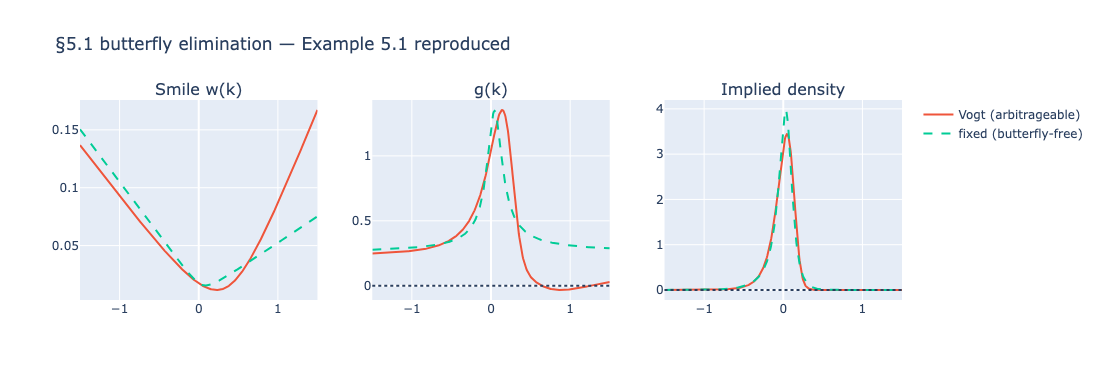
\includegraphics[
        width=0.95\textwidth,
        trim=0 0 0 2.5cm,
        clip
    ]{figures/nb02_c19_0.png}
    \caption{The Vogt smile (Example~\ref{ex:vogt}) and its repair, as computed in NB02.
    Left to right: total variance $w(k)$, the Durrleman function $g(k)$, and the implied density.
    The Vogt slice (solid) looks innocuous in total variance yet has $\min_k g=-0.0329$, so its
    density turns negative: a genuine butterfly arbitrage invisible to the eye. Butterfly
    elimination in Jump--Wings space (paper~\S5.1), holding $(v_t,\psi_t,p_t)$ and moving
    $(c_t,\tilde v_t)$ to the arbitrage-free boundary, gives the repaired slice (dashed), which
    restores $g\ge0$ and a nonnegative density, lifting $\min_k g$ to $+0.2704$.}
    \label{fig:nb02vogt}
\end{figure}



\paragraph{Quasi-explicit calibration.} The slice calibrator follows the quasi-explicit
decomposition of \cite{gatheraljacquier2014}: an outer Nelder--Mead search over the two
nonlinear parameters $(m,\sigma)$, and, for each candidate, an inner constrained linear
least-squares fit of the three parameters on which $w$ depends linearly once $(m,\sigma)$ is
fixed, subject to the paper's domain bounds. On a synthetic slice it recovers
$\mathrm{RMSE}(w)=2.8\times10^{-4}$, with $\min_k g=0.44$ on the quoted range and $0.31$ on the
wider range $k\in[-2,2]$.

\begin{figure}[htbp]
    \centering
    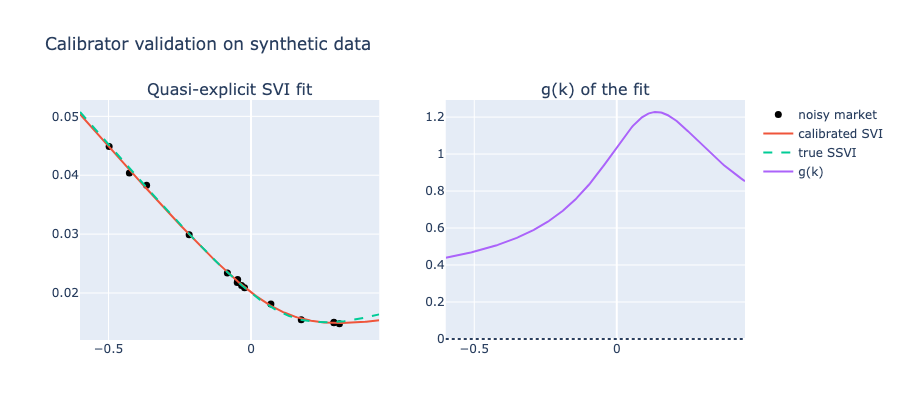
\includegraphics[
        width=0.9\textwidth,
        trim=0 0 0 2.5cm,
        clip
    ]{figures/nb02_c13_0.png}
    \caption{Quasi-explicit SVI calibrator validated on synthetic data: recovered slice against
    ground truth, $\mathrm{RMSE}(w)=2.8\times10^{-4}$. Source: Notebook~02, cell~13.}
    \label{fig:nb02calib}
\end{figure}



\paragraph{SSVI variants and certificates.} Propositions~\ref{thm:gjcal}--\ref{thm:gjbfly} are
implemented as executable certificates and verified on the paper's three $\varphi$ families, the
power-law, Heston-like, and globally guaranteed modified power law of
Example~\ref{ex:phifamilies}, all passing with the published condition values
\notebookfig{02}{SSVI phi families: certificate table}. The arbitrage-free interpolation and
extrapolation of \eqref{eq:interp}--\eqref{eq:interp2} are verified numerically: the interpolated
slice attains $\min_k g=0.52$, and the extrapolated slice dominates the last calibrated slice
everywhere (Figure~\ref{fig:nb02interp}, top). Finally, a crossedness penalty
(\cite[Def.~5.1]{gatheraljacquier2014}) added to the SSVI objective drives total crossedness from
$0.113$ to $0.000$ on a stressed synthetic term structure.


\begin{figure}[htbp]
    \centering
    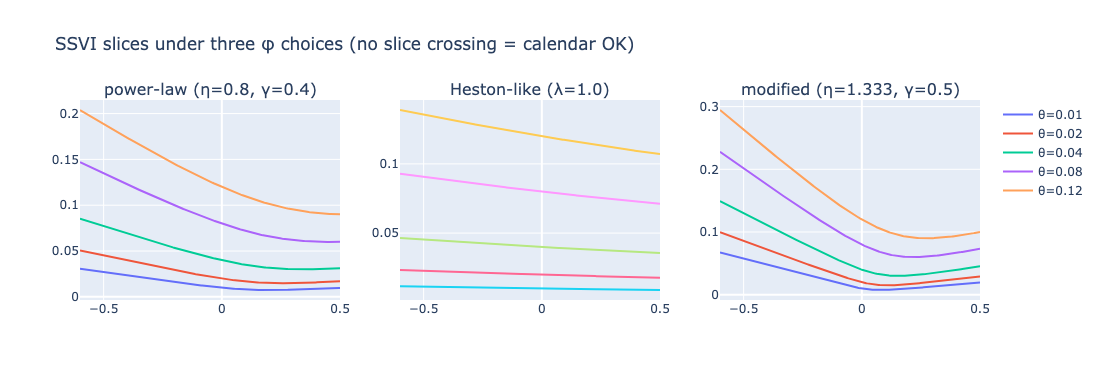
\includegraphics[
        width=0.9\textwidth,
        trim=0 0 0 2.5cm,
        clip
    ]{figures/nb02_c22_0.png}\\[0.1ex]
    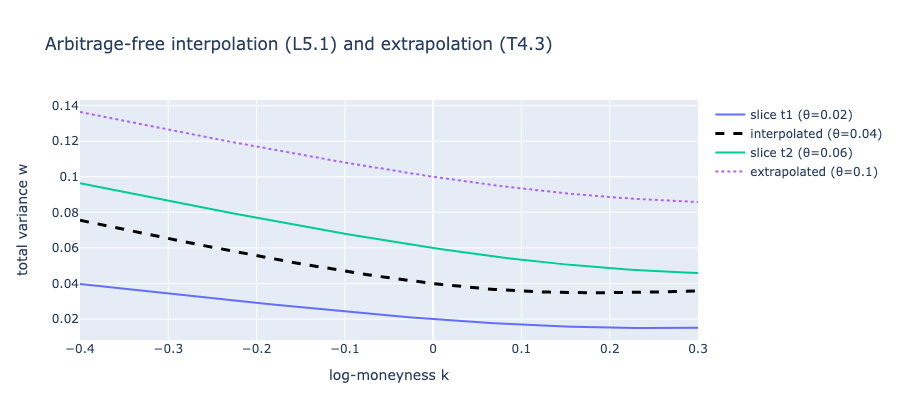
\includegraphics[
        width=0.90\textwidth,
        trim=0 0 0 2.5cm,
        clip
    ]{figures/nb02_c25_0.png}\\[0.1ex]
    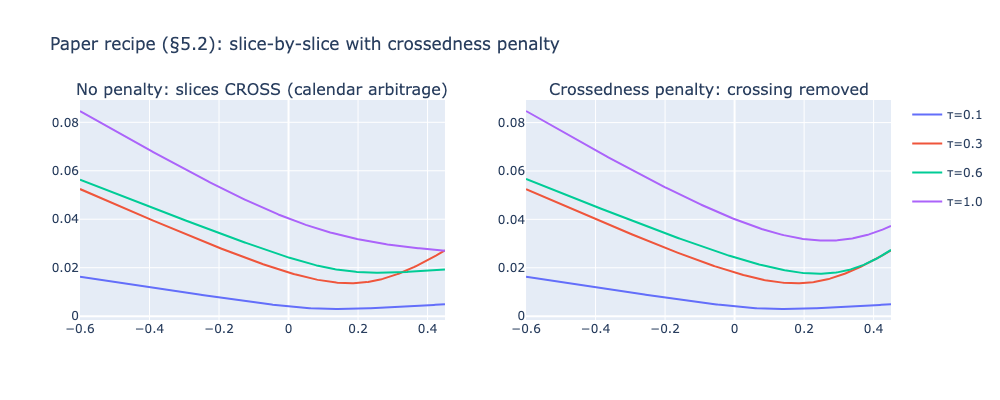
\includegraphics[
        width=0.95\textwidth,
        trim=0 0 0 2.5cm,
        clip
    ]{figures/nb02_c16_1.png}
    \caption{SSVI construction and its arbitrage-free operations.
    \textbf{Top:} under each of the three $\varphi$ families the slices never cross, so the surface
    is calendar-arbitrage-free by construction (Proposition~\ref{thm:gjcal}).
    \textbf{Middle:} arbitrage-free interpolation and flat extrapolation; the interpolated slice
    reaches $\min_k g=0.52$ and the extrapolated slice dominates the last calibrated one everywhere.
    \textbf{Bottom:} calendar repair by a crossedness penalty (paper~\S5.2) on a stressed synthetic
    term structure in which one short-maturity slice has been inflated to force a crossing. Without
    the penalty (left) adjacent slices cross, with total crossedness $0.113$; with the penalty
    (right) it is driven to $0.000$. Near the right edge the $\tau=0.3$ and $\tau=0.6$ slices
    approach closely but do not cross, the shorter staying below the longer everywhere
    ($\max_k(w_{0.3}-w_{0.6})=-1.9\times10^{-3}<0$).}
    \label{fig:nb02interp}
\end{figure}

% préambule : \usepackage{placeins}

\subsection{Benchmark methodology and results on real data}\label{sec:parametricreal}

The same machinery is now run on real SPX quotes. For each trading day we fit two objects: a
\emph{per-slice} SVI surface (quasi-explicit calibration, with inverse-spread and IV-target
weights) and a \emph{surface-wide} SSVI (weighted symmetrically across slices; an earlier
asymmetric weighting that disadvantaged SSVI was removed once identified). Each day is then put
through the full protocol: the $\mathrm{crc32}$ hold-out of Section~\ref{sec:protocol},
$g$-audits on both the quoted and the wide grids, slice crossedness, and the paper's two repair
procedures applied to the \emph{real} fits, butterfly elimination (\S5.1) and calendar refit
under a crossedness penalty (\S5.2).

The numbers below come from a preliminary eight-day January-2018 sample. The full 2018--2025
production run replaces them at submission; the pipeline is identical, invoked with
\texttt{LIMIT\_DATES=None}, and every staging-scale entry is marked $^\dagger$.

\begin{table}[htbp]\centering\small
\caption{Parametric benchmark on the full quoted domain (8 days$^\dagger$, 258 slices). Hold-out
follows the $\mathrm{crc32}$ protocol shared by all chapters.
\notebookfig{02}{benchmark summary table}}
\label{tab:nb02}
\begin{tabular}{lcc}
\toprule
 & SVI (per slice) & SSVI (surface) \\
\midrule
In-sample RMSE (\vp)        & $0.635^\dagger$ & $1.957^\dagger$ \\
Hold-out RMSE (\vp)         & $0.640^\dagger$ & $1.913^\dagger$ \\
Butterfly-violating slices  & $12.0\%$ / $11.2\%$ (quoted/wide)$^\dagger$ & $0\%$ (certified) \\
Median crossedness          & $2.1\times10^{-2\,\dagger}$ & $0$ (by construction) \\
\bottomrule
\end{tabular}
\end{table}

\begin{table}[htbp]\centering\small
\caption{Full-domain results by maturity bucket$^\dagger$. Butterfly violations concentrate at
the ultra-short end and, there, in the core moneyness region: all $16/16$ minimisers of $g$ lie
in $k\in[-0.6,0.4]$. This is a structural limitation of the SVI form where $w$ is small and the
$1/w$ term of \eqref{eq:g} amplifies the convexity of the fit.
\notebookfig{02}{fit and violations by maturity bucket}}
\label{tab:buckets}
\begin{tabular}{lccc}
\toprule
Maturity bucket & Median RMSE (\vp) & Violations & Slices \\
\midrule
7--14\,d   & 0.995 & 55.2\% & 29 \\
15--60\,d  & 1.003 & 0.0\%  & 109 \\
61--180\,d & 0.881 & 0.0\%  & 56 \\
$>$180\,d  & 0.135 & 0.0\%  & 64 \\
\bottomrule
\end{tabular}
\end{table}

\FloatBarrier
Three findings organise the section.

\paragraph{The fit--arbitrage trade-off is a number.} Per-slice SVI reaches $0.64\,\vp$ on
held-out quotes, the best fit in the study, but it leaks butterfly arbitrage on $12\%$ of slices
and carries non-zero crossedness between adjacent slices: fitting each maturity independently
buys accuracy at the cost of surface coherence. SSVI, certified arbitrage-free by
Theorem~\ref{lem:range}, pays roughly three times the error for that guarantee. The interval
$[0.64,\,1.91]\,\vp$ is thus the window every learning method must enter, cheaper than SSVI yet
cleaner than per-slice SVI.

\paragraph{Difficulty is localised, and not where one would expect.} Table~\ref{tab:buckets}
shows that violations are almost entirely an ultra-short-maturity phenomenon: $55\%$ of $7$--$14$
day slices violate, against $0\%$ everywhere beyond two weeks. Within those short slices the
violations sit in the \emph{core} moneyness region, not in the wings. The practical consequence
is counter-intuitive: restricting the moneyness range does not clean the data, whereas the
$\mathrm{DTE}\ge10$ maturity filter does (Figure~\ref{fig:nb02buckets}).

\begin{figure}[htbp]
    \centering
    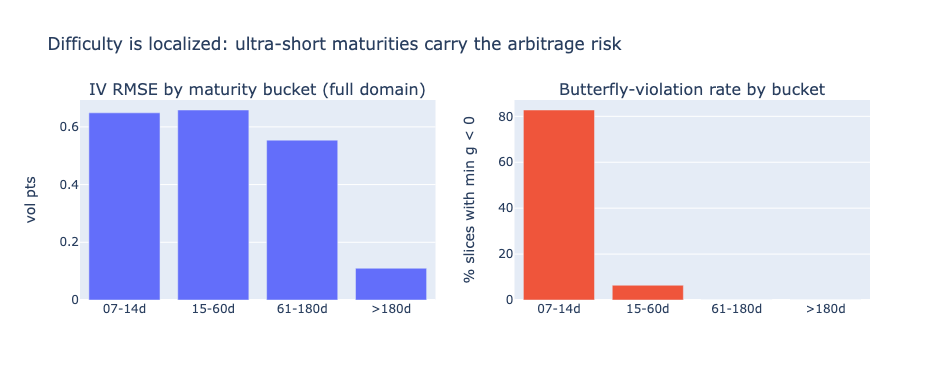
\includegraphics[
        width=0.82\textwidth,
        trim=0 0 0 2.5cm,
        clip
    ]{figures/nb02_c37_1.png}
    \caption{Median fit error and butterfly-violation rate by maturity bucket on the full domain
    (Table~\ref{tab:buckets}); violations are confined to the ultra-short end. Source:
    Notebook~02, cell~37.}
    \label{fig:nb02buckets}
\end{figure}

\begin{figure}[htbp]
    \centering
    
\includegraphics[
        width=0.82\textwidth,
        trim=0 0 0 3.5cm,
        clip
    ]{figures/nb02_c39_0.png}
    \caption{Median IV RMSE under the full and paper evaluation domains, in-sample and hold-out.
    Restricting the moneyness range leaves the error essentially unchanged; the maturity filter
    is what removes the violating slices. Source: Notebook~02, cell~39.}
    \label{fig:nb02domains}
\end{figure}


\FloatBarrier

\paragraph{The benchmark matches the industrial reference.} Evaluating our per-day SVI fits on
the grid of the proprietary OptionMetrics volatility surface gives a median absolute gap of
$0.93\,\vp$ over $2{,}958$ grid points, with a $90$th percentile of $3.13\,\vp$: a fully
transparent pipeline reproduces the commercial smoother to within one volatility point at the
median. Repairing the real fits with the paper's recipes is, by contrast, expensive: a median
$+4.2\,\vp$ for butterfly elimination ($31/31$ violating slices cured on the quoted domain) and
$+0.15\,\vp$ for the calendar refit. \emph{Ex-post repair costs several volatility points}, which
is the case for building the constraints into training instead, exactly what
Section~\ref{sec:deep} attempts, and where the thesis's central finding lives.\\

A single representative day makes the two failure modes concrete
(Figures~\ref{fig:nb02day} and~\ref{fig:nb02crossing}): the fits themselves, and the calendar
crossings between adjacent per-slice SVIs that SSVI avoids by construction.

\begin{figure}[htbp]
    \centering
    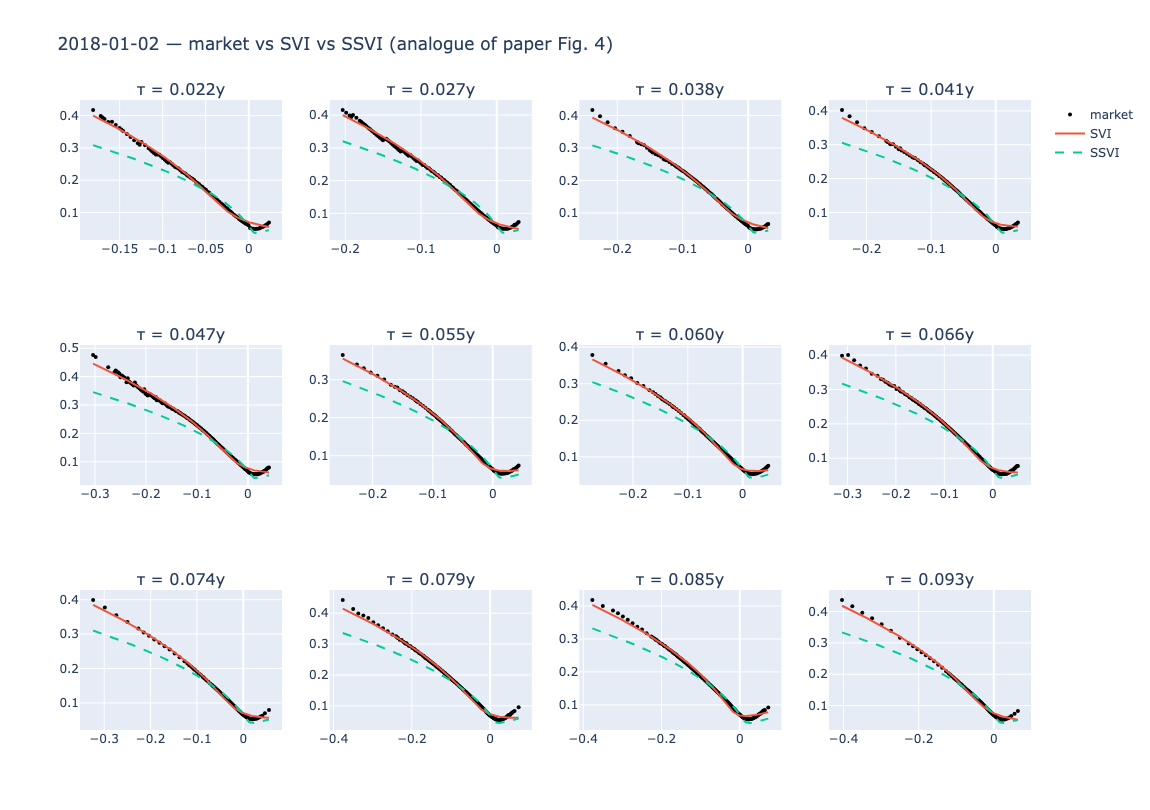
\includegraphics[
        width=1.10\textwidth,
        trim=0 0 0 2.5cm,
        clip
    ]{figures/nb02_c41_0.png}
    \caption{One representative trading day: market quotes (dots) with the per-slice SVI fit
    (solid) and the surface SSVI fit (dashed), the analogue of the paper's Fig.~4. Source:
    Notebook~02, cell~41.}
    \label{fig:nb02day}
\end{figure}

\begin{figure}[htbp]
    \centering
    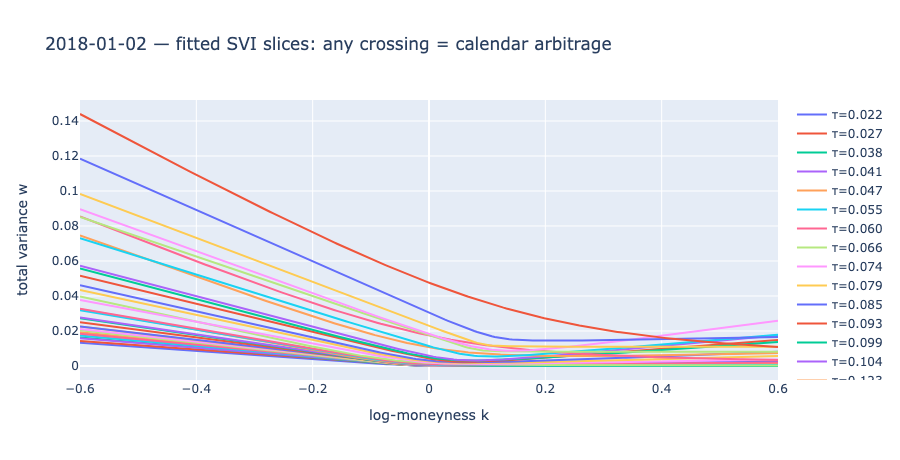
\includegraphics[
        width=1.10\textwidth,
        trim=0 0 0 2.5cm,
        clip
    ]{figures/nb02_c43_0.png}
    \caption{The same day's fitted SVI slices in total variance; any crossing is a calendar
    arbitrage between adjacent per-slice fits, the surface incoherence that SSVI avoids by
    construction. Source: Notebook~02, cell~43.}
    \label{fig:nb02crossing}
\end{figure}


\FloatBarrier

The worst slice in the sample (Figure~\ref{fig:nb02worst}) is the live-data counterpart of the
Vogt smile of Example~\ref{ex:vogt}, and it is the stress candidate carried forward to
Section~\ref{sec:deep}.

\begin{figure}[htbp]
    \centering
    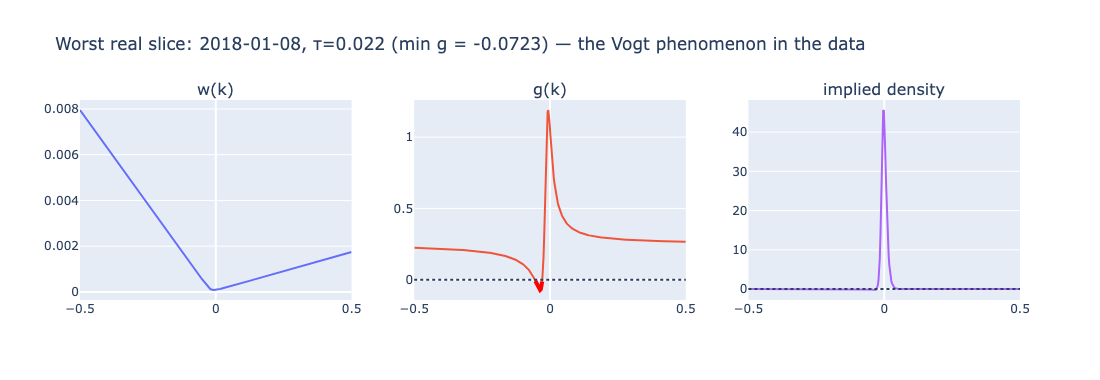
\includegraphics[
        width=0.99\textwidth,
        trim=0 0 0 2.5cm,
        clip
    ]{figures/nb02_c45_0.png}
    \caption{The worst real slice in the sample (2018-01-08, $\tau=0.022$, $\min_k g=-0.072$):
    the Vogt phenomenon in live SPX data, and the ex-ante stress candidate used in
    Section~\ref{sec:deep}. Source: Notebook~02, cell~45.}
    \label{fig:nb02worst}
\end{figure}


\FloatBarrier

% ============================================================================
\section{Derivative-constrained deep smoothing and the collocation blind spot}
\label{sec:deep}
% ============================================================================

\subsection{Method}

\paragraph{Architecture.} Following \cite{ackerer2020}, the surface is the multiplicative
prior--corrector model \eqref{eq:arch}: an SSVI prior with power-law term structure fitted to
the day's quotes, multiplied by a positive corrector ($2\times64$ tanh units, inputs rescaled
to $[-1,1]^2$, and $\approx1$ at initialisation so that training \emph{starts at the prior}).
The prior is calibrated with a robust nearest-ATM proxy followed by a joint five-parameter
Nelder--Mead refinement, constrained to stay \emph{inside} the Gatheral--Jacquier region. By
Theorem~\ref{lem:range} the fitted prior therefore carries a printed certificate; for the
synthetic experiments it reads $\theta_{\max}=0.062$ with condition values $0.28<4$ and
$0.83\le4$ \notebookfig{03}{GJ certificate log}.

\paragraph{Objective.} The loss is \eqref{eq:loss} with $\lambda_{\mathrm b}=\lambda_{\mathrm
c}=10$ and $\lambda_{\mathrm w}=0.1$. Fit weights are IV-targeted,
$\omega_i\propto1/(4w_i\tau_i)$, so that by the delta method a least-squares problem in $w$
approximates a least-squares problem in implied volatility. These are the same weights as the
calibrators of Section~\ref{sec:parametric}, the symmetry the cross-family comparison
requires. All surface derivatives entering the penalties are obtained by exact automatic
differentiation and validated against closed forms.

\subsection{Equal-epoch ablations on synthetic ground truth}

Ground truth is a known SSVI surface; the quotes are sparse (54 over six maturities),
irregular and noisy; and the prior is \emph{refit from the quotes}, so it is deliberately
misspecified and the corrector has genuine work to do. Four variants train for the \emph{same}
number of epochs with persistent optimizer state. An earlier version re-initialised Adam at
every logging chunk and reported all final metrics mid-restart-transient, which is why the
equal-epoch protocol is stated explicitly here.

\begin{table}[htbp]\centering\small
\caption{Equal-epoch ablation ($800$ epochs). RMSE is measured against the dense truth at the
quoted maturities; the audit uses the independent extended grid.
\notebookfig{03}{equal-epoch dynamics}}
\label{tab:ablation}
\begin{tabular}{lccc}
\toprule
Variant & RMSE (\vp) & $\min g$ (audit) & bfly / cal violations \\
\midrule
full (prior $+$ penalties)  & 0.096 & $+0.310$ & 0\% / 0\% \\
no constraints              & 0.094 & $+0.311$ & 0\% / 0\% \\
no prior ($+$ penalties)    & 1.060 & $+0.268$ & 0\% / 0\% \\
no prior, no constraints    & 1.060 & $+0.268$ & 0\% / 0\% \\
\midrule
prior only (no corrector)   & 0.154 & --- & 0\% / 0\% \\
\bottomrule
\end{tabular}
\end{table}

Table~\ref{tab:ablation} contains two deliberate curiosities. First, the two \emph{no-prior}
rows are identical to the last digit, and their training traces coincide exactly
(Figure~\ref{fig:nb03dynamics}). This is the finding, not a copy-paste error: on clean data
$g_\theta>0$ holds throughout training, so $\relu(-g_\theta)^2$ and its gradient vanish
\emph{exactly}, and the penalised and unpenalised runs follow the same trajectory. Second, the
certified prior carries the accuracy: $0.154\,\vp$ for the prior alone, $0.096\,\vp$ once the
corrector is added, against $1.06\,\vp$ without any prior. On clean data the prior does the
protective work and the penalties are dormant. This raises the obvious question, do the
penalties do anything at all, and to answer it the data must \emph{demand} arbitrage.

\begin{figure}[htbp]
    \centering
    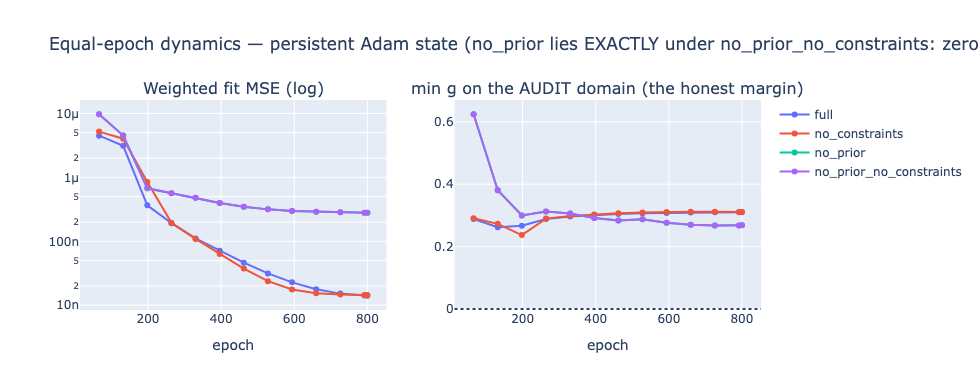
\includegraphics[
        width=0.92\textwidth,
        trim=0 0 0 2.5cm,
        clip
    ]{figures/nb03_equal_epoch_dynamics.png}
    \caption{Equal-epoch training dynamics. The \texttt{no\_prior} trace lies exactly under
    \texttt{no\_prior\_no\_constraints}: with $g_\theta>0$ throughout, the penalty gradient is
    identically zero and the two runs are indistinguishable. Source: Notebook~03.}
    \label{fig:nb03dynamics}
\end{figure}

\FloatBarrier

\subsection{A stress test that is guaranteed, fittable and gated}\label{sec:stress}

\paragraph{Design.} We deflate the \emph{last} maturity slice by a factor $0.45$. Since
$0.45<\theta(0.9)/\theta(1.4)=(0.9/1.4)^{0.95}\approx0.657$, the deflated quotes sit strictly
below those of the previous maturity, so \emph{any} surface fitting both must have
$\partial_\tau w<0$ somewhere between them; the data-level crossing is $+0.0290$ in $w$. The
stressor is thus verified \emph{analytically} to force the pathology rather than assumed to.
Deflation is chosen over inflation for two reasons: the IV-target weights
$\propto1/(4w\tau)$ \emph{raise} the stressed slice's weight, and the corrector feature
required to follow it is low-frequency, which a tanh MLP learns readily. A synthetic
\emph{butterfly} stressor is deliberately absent, because at short maturities $g<0$ is driven
by the slope term $w'^2/(4w)$ with tiny $w$ and would require distortions sharper than a
smooth prior-times-corrector can produce at fittable widths. The butterfly penalty is instead
ablated on real ultra-short quotes in Section~\ref{sec:realablation}.

\paragraph{The gate.} A stress comparison is interpretable only if the models actually
\emph{fit} the stressor, since an unfitted stressor produces non-convergence noise dressed as
an arbitrage result. Validity is therefore verified rather than assumed, by a two-condition
gate on the unconstrained model: (a)~the deflated-slice RMSE is below $1\,\vp$, and (b)~the
fitted surface itself reproduces at least half the data-level crossing. Condition (a) alone
would be insufficient, since a surface can graze the deflated slice from above without ever
crossing. On the final run the gate reads \texttt{PASS/PASS}, with $0.069\,\vp$ and a fitted
crossing of $+0.0296$ against $+0.0290$ in the data \notebookfig{03}{fit-validity gate log}.

\subsection{The blind spot: exhibit, mechanism, repair}\label{sec:blindspot}

\paragraph{Exhibit.} On this gated stress, an early version of the smoother produced, for the
\emph{constrained} model ($\lambda=10$), the pair of numbers that reorganised the thesis:
\[
\texttt{pen\_cal}\big|_{\hat X_{\mathrm c}}=0.000\times10^{0}
\qquad\text{and}\qquad
\text{audit-grid calendar violations}=28\% .
\]
Both were true. Diagnostics excluded the optimizer, since the constrained run had the
\emph{lower} total loss under its own objective, and excluded the automatic differentiation,
since the $\tau$-path gradient was $\|\nabla\texttt{pen\_cal}\|=0.25$ at a violating point and
the $\tau$-derivative validated to $10^{-11}$. What remained was the grid.

\paragraph{Mechanism.} The collocation followed the literature's prescription: exponentially
spaced maturities, dense at the short end where the butterfly constraint bites because $w$ is
small \cite{ackerer2020}. With ten nodes on $[0.06,1.4]$ that grid reads
$0.060,\,0.085,\,\dots,\,0.696,\,0.987,\,1.400$, so there is \emph{no node at all} between
$0.987$ and $1.400$: a $0.41$-year hole covering $30\%$ of the maturity axis
(Figure~\ref{fig:gridhole}), exactly where the stressor forces the crossing. The optimizer
satisfied the penalty at every node and let the surface dip between them, which is precisely
the extremal configuration of Theorem~\ref{prop:nodegap}, and the penalty reported zero in
perfect good faith. The two constraints have \emph{opposite} grid requirements
(Section~\ref{sec:softtheory}), so serving both with one exponential grid silently disarms the
calendar penalty at the long end. This is \cite{chataigner2020}'s caveat in its most literal
form, and it was detectable only because the audit grid is independent of, and finer than, the
collocation grid (Remark~\ref{rem:sampling}).

\paragraph{Repair: constraint-specific collocation.} The butterfly penalty keeps its ATM-dense
grid (cube-root $k$ spacing, hybrid exponential-union-uniform $\tau$, maximal gap $0.10$y).
The calendar penalty, which costs only one first derivative per node, gets its own
uniform-dense $\tau$ grid of $80$ nodes with maximal gap $0.017$y. By
Theorem~\ref{prop:nodegap} this is roughly a $24$-fold reduction of the worst admissible
hidden violation at equal curvature. A resolution assertion verifies, before any stress run,
that the calendar grid can actually \emph{see} the stressed interval.

\begin{table}[htbp]\centering\small
\caption{Calendar stress, $\lambda$-sweep (final run, gated). ``mat'' denotes material
violations at $\mathrm{tol}_{\mathrm{mat}}=10^{-3}$ (Definition~\ref{def:materiality}). Node
and audit penalties now agree to grid noise: the blind spot is closed.
\notebookfig{03}{lambda sweep log}}
\label{tab:sweep}
\begin{tabular}{lcccc}
\toprule
$\lambda$ & deflated fit (\vp) & fitted crossing & cal.\ viol.\ strict (mat) & pen.\ nodes / audit \\
\midrule
0  & 0.069 & $+0.0296$ & 34.7\% (34.4\%) & $1.35\text{e-}3$ / $1.29\text{e-}3$ \\
1  & 1.991 & $+0.0000$ & 4.4\% (0.0\%)   & $1.3\text{e-}9$ / $1.2\text{e-}9$ \\
10 & 1.963 & $-0.0002$ & 1.6\% (0.0\%)   & $8.4\text{e-}11$ / $1.2\text{e-}10$ \\
\bottomrule
\end{tabular}
\end{table}

\paragraph{Result.} Table~\ref{tab:sweep} is the Ackerer trade-off made visible and
trustworthy. The unconstrained model follows the deflated quotes down, with a fitted crossing
of $+0.0296$ and material violations on a third of the audit domain; the constrained model
\emph{refuses}, with a fitted crossing of $-0.0002$, at a measured price of about $1.9\,\vp$
on the deflated slice. Material violations fall from $34.4\%$ to $0.0\%$
(Figure~\ref{fig:nb03stress}). The residual \emph{strict} rate of $1.6\%$, whose deepest
residual is $\partial_\tau w=-1.3\times10^{-4}$, is the honest signature of the soft-constraint
approach: reduced but not abolished, and now \emph{sized} rather than merely counted. The
earlier, magnitude-inconsistent blind-spot detector false-alarmed on exactly this residual,
whereas the material-scale detector of Definition~\ref{def:materiality} is silent here and
loud on the true pathology.

\begin{figure}[htbp]
    \centering
    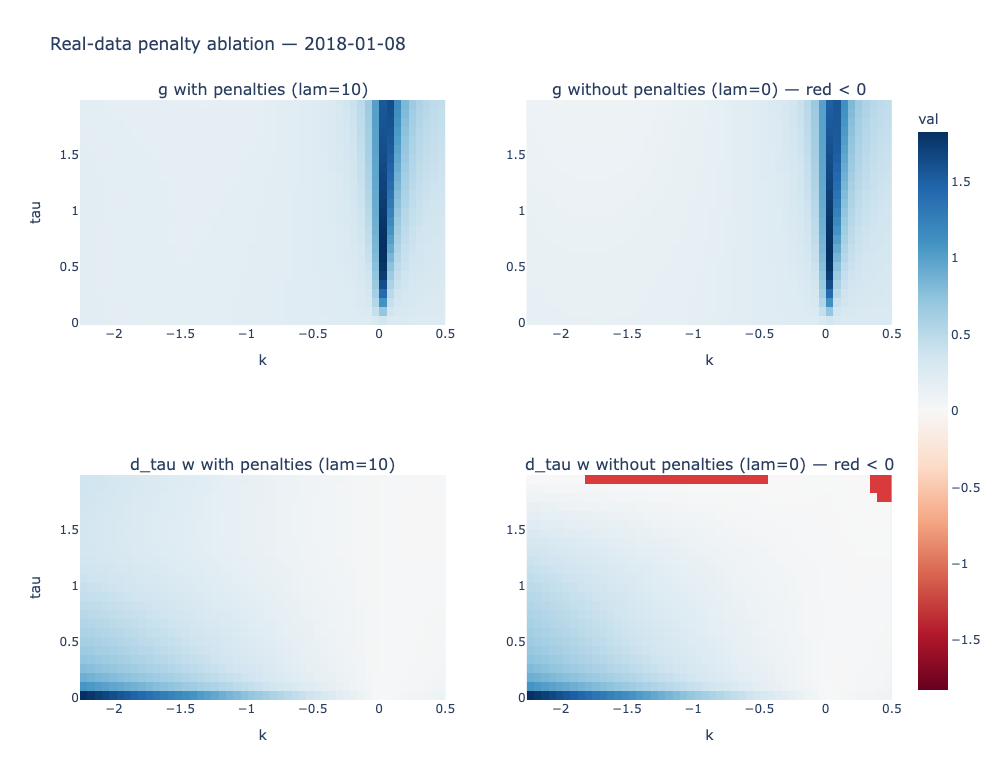
\includegraphics[
        width=0.92\textwidth,
        trim=0 0 0 2.5cm,
        clip
    ]{figures/nb03_stress_A.png}
    \caption{The calendar stress under both regimes. The $\partial_\tau w$ maps with the audit
    overlay show the unconstrained surface dipping negative across the long-end hole, and the
    constrained surface holding $\partial_\tau w\ge0$ there; the arbitration at the money makes
    the $1.9\,\vp$ price of that refusal explicit. Source: Notebook~03.}
    \label{fig:nb03stress}
\end{figure}
\FloatBarrier

\begin{finding}[The collocation blind spot]\label{find:blindspot}
A soft no-arbitrage penalty is a statement about its sampling set. A grid optimal for one
constraint can be structurally blind to another, the failure is invisible to the training loss
exactly, and it is detectable only by an audit grid independent of every collocation grid,
compared on a materiality scale. Constraint-specific collocation closes it.
\end{finding}

\subsection{Robustness to sparsity, and two instructive leaks}\label{sec:sparsity}

Subsampling the quotes from $100\%$ to $50\%$ and then $25\%$, against per-slice SVI, exposed
in sequence two failures of \emph{our own} experimental design. Both are reported because each
produced an impossible number that acted as its own alarm.

\paragraph{Leak 1: data.} The first version reused the prior, the collocation and the input
scaling calibrated on the \emph{full} quote set inside the subsampling loop. Since the prior
carries most of the surface (Table~\ref{tab:ablation}), the deep model kept seeing quotes that
SVI was denied, and its RMSE \emph{fell} as $74\%$ of the data was removed. An error rate that
improves as data is destroyed is impossible, and that is what flagged the leak.

\paragraph{Leak 2: estimator.} With the leak closed, one $50\%$ draw exploded to $14.2\,\vp$.
The naive ATM interpolation inside the prior fit \emph{clamps} on one-sided slices, corrupting
$\theta(\tau)$; and for a multiplicative corrector a \emph{wrong} prior is worse than a
\emph{flat} one ($14.2$ against $1.7\,\vp$), because the corrector must first spend capacity
undoing it, as the log-decomposition of \eqref{eq:arch} predicts. The robust
nearest-ATM calibrator with joint refinement fixed it, and the study became multi-seed with
the prior-only RMSE printed for every draw, the diagnostic that separates prior failures from
corrector failures.

\paragraph{Final numbers.} Medians over seeds: the deep smoother degrades gracefully,
$0.096\to0.22\to0.34\,\vp$ as quotes fall from $100\%$ to $50\%$ to $25\%$, bounded below by
the prior-only curve. SVI first loses accuracy and then \emph{coverage}: at $25\%$ no slice
retains the six quotes a five-parameter SVI needs, and it returns nothing at all. Because
SVI's RMSE is conditional on a calibrability set that itself changes with the subsampling
fraction, connecting its medians across fractions would manufacture the artifact ``SVI
improves under sparsity''. The comparison is therefore \emph{paired} on the same slices, draw
by draw: the deep smoother wins $4/4$ paired draws, including $0.137$ against $1.615\,\vp$.
One $25\%$ draw still degrades to $1.68\,\vp$, and its prior-only column of $1.21\,\vp$
convicts the prior rather than the corrector.
\notebookfig{03}{sparsity: accuracy panel and paired deep-vs-SVI panel}

\begin{finding}[Sparsity robustness is inherited]\label{find:sparsity}
The deep smoother's robustness to sparse quotes is inherited from the calibration robustness
of its prior. The prior-times-corrector architecture moves the failure point; it does not
remove it.
\end{finding}

\subsection{Real SPX days and the penalty ablation}\label{sec:realablation}

The per-day driver reuses the NB02 protocol: per-\texttt{exdate} hold-out, symmetric weights,
day-specific constraint-specific grids, capped-extended audit, and a GJ-certified prior whose
per-day certificate and prior-only RMSE are both stored. It was staged on early-January 2018
days together with an \emph{ex-ante} stress candidate selected from
Section~\ref{sec:parametric}'s audit, namely 2018-01-08, which carries six butterfly-violating
SVI slices on the wide grid with $\min_k g=-0.071$ (Figure~\ref{fig:nb02worst}). Staging
results are a hold-out of $1.70$--$1.81\,\vp$, zero strict violations on both the quoted and
extended domains, no blind flags, and green certificates.

The $\gamma\le\tfrac12$ episode of Remark~\ref{rem:cert} was diagnosed on these same days, the
per-day prior-only RMSE being what localised it, and the endpoint certification recovers the
free fit: hold-out on the same days improves to $1.15$--$1.31\,\vp$ under the free-$\gamma$
run.

\begin{figure}[htbp]
    \centering
    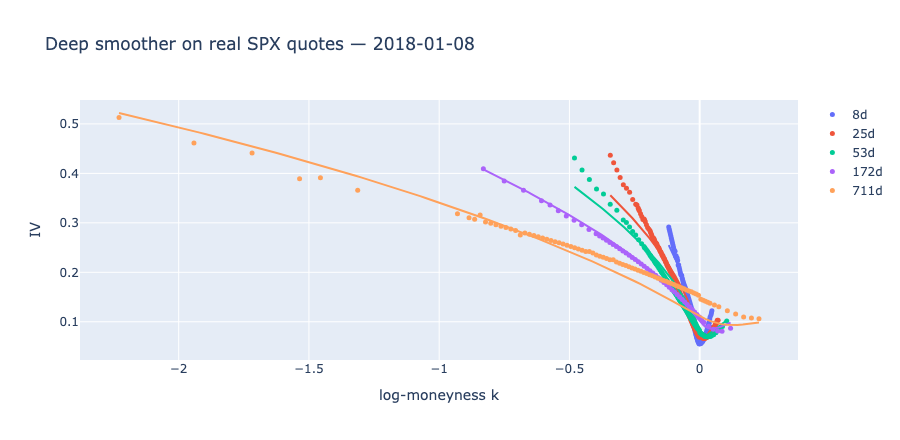
\includegraphics[
        width=0.9\textwidth,
        trim=0 0 0 2.5cm,
        clip
    ]{figures/nb03_real_spx_quotes.png}
    \caption{The deep smoother on real SPX quotes, 2018-01-08: market quotes with the fitted
    surface, on the day carrying the worst butterfly violation of the parametric benchmark.
    Source: Notebook~03.}
    \label{fig:nb03real}
\end{figure}

\begin{figure}[htbp]
    \centering
    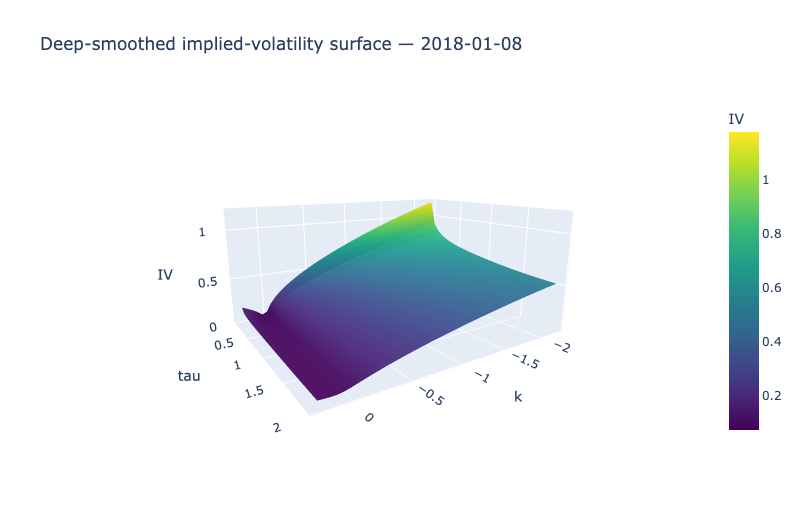
\includegraphics[
        width=0.9\textwidth,
        trim=0 0 0 2.5cm,
        clip
    ]{figures/nb03_deep_smoothed_surface.png}
    \caption{The corresponding deep-smoothed implied-volatility surface for 2018-01-08.
    Source: Notebook~03.}
    \label{fig:nb03realsurface}
\end{figure}

\FloatBarrier

\paragraph{Which constraint binds on real data?} Refitting the stress-candidate day with
$\lambda_{\mathrm b}=\lambda_{\mathrm c}=0$, at identical seed, hold-out and epoch budget,
answers the question. The butterfly penalty \texttt{pen\_bfly} is \emph{identically zero at
both} values of $\lambda$: with the certified prior the surface never goes butterfly-negative
even when unconstrained, so NB02's $55\%$ figure is a statement about raw per-slice SVI, not
about this architecture. The binding real constraint is the \emph{calendar} one. On
2018-01-03, $\lambda=0$ leaves $19.1\%$ of the extended domain violating with
$\min\partial_\tau w=-0.25$, against $0.0\%$ at $\lambda=10$; while on the most
butterfly-stressed day, 2018-01-08, even the calendar penalty is dormant and the prior alone
suffices \notebookfig{03}{real-data penalty ablation quadrant}. The hypothesis that real
ultra-short quotes are the natural butterfly stressor is thereby downgraded to a question for
the full five-year run, answerable from the per-day audit columns, with the Volmageddon and
COVID weeks the natural suspects.

One optimisation curiosity is flagged rather than exploited. At equal epoch budget,
$\lambda=0$ fits slightly \emph{worse} in-sample, which is impossible at the optimum since it
minimises a strict subset of the loss terms. It is therefore an optimisation artefact, the
penalties preconditioning the descent, and it is explicitly \emph{not} reported as
``constraints improve accuracy''.

% ============================================================================
\section{Operator deep smoothing: one model for every surface}\label{sec:operator}
% ============================================================================

Section~\ref{sec:deep} fits one network per day; this section learns the smoothing \emph{map}
itself. Following \cite{wiedemann2025}, an operator $\mathcal G_\vartheta$ consumes a day's
irregular quote cloud $\{(k_i,\tau_i,\sigma_{\mathrm{IV},i})\}$ and returns
$\widehat\sigma_{\mathrm{IV}}$ at \emph{any} query point, for \emph{any} day, with no per-day
optimisation (Section~\ref{sec:opsec}). Three questions organise the section. What does the
operator programme deliver in the \emph{academic-data} regime, one index and $1{,}926$ days,
against the reference paper's decade of proprietary multi-asset data? Does synthetic
pretraining on SSVI-generated surfaces close the gap? And do the operator's soft constraints
survive the audit methodology of Finding~\ref{find:blindspot}?

\subsection{Design}

\paragraph{Data and split.} The real bank holds $1{,}926$ days (2018-01-02 to 2025-08-29,
with $2{,}367$--$2{,}500$ quotes per day after capping), split \emph{chronologically} into
$1{,}155/385/386$ days for training, validation and test. The test set is the genuinely
out-of-sample final year and a half, so every test number below is a temporal generalisation
claim rather than an in-sample one. The synthetic bank holds $1{,}000$ SSVI surfaces with
randomly drawn certified parameters and irregular quote configurations of $48$ to $201$
quotes, providing an unlimited and arbitrage-free pretraining source.

\paragraph{Two architectures, three regimes.} We train a DeepONet-class operator
\eqref{eq:deeponet} (set encoder into branch, coordinates into trunk; $67{,}009$ parameters)
and a graph-neural-operator variant \eqref{eq:gno} (message passing from the $m$ nearest
quotes to each query; $34{,}697$ parameters). Each is trained under three regimes:
\textbf{R1} real-only, \textbf{R2} synthetic-only with zero-shot transfer to real data, and
\textbf{R3} synthetic pretraining followed by real finetuning. Losses follow \eqref{eq:loss}
with vega-clamped relative fit weights, and butterfly and calendar penalties resolved by
finite differences on a $22\times9$ grid. That coarse grid is \emph{deliberately kept} as in
the reference design, because the gap between what it sees and what an independent audit sees
is itself one of this thesis's measurements (Section~\ref{sec:opaudit}).

\paragraph{Two engineering failures worth reporting.} The first is a \emph{dying softplus}.
The DeepONet trained from scratch on real data collapsed to a constant: the training loss sat
at exactly $1.0000$, the value of the relative loss for a zero prediction, and the audit
returned $\min g=0.9995$, which is the value $g\equiv1$ takes for a surface flat in $k$
(set $w'=w''=0$ in \eqref{eq:g}), up to the audit's discretisation. Real SPX days are
dominated by far-OTM puts whose near-zero vegas explode the normalised fit weights; the
pre-activation is driven far negative early in training and the softplus gradient vanishes.
Output-bias initialisation at $\mathrm{softplus}^{-1}(0.20)$, a weight cap and a lower
learning rate cure it. The second failure is \emph{vacuous invariance}: the collapsed model
displayed \emph{perfect} discretization invariance, because a constant is trivially invariant
to its inputs (Definition~\ref{def:discinv}). The invariance study is therefore \emph{gated}
on fit validity, requiring a day RMSE below $5\,\vp$, the same epistemic move as the stress
gate of Section~\ref{sec:stress}: a metric computed on a model that cannot fit is vacuous and
must be excluded, not reported. \notebookfig{04}{training curves per family and regime}

\subsection{Accuracy and transfer}

On the $386$ out-of-sample days the graph operator is the accuracy leader, reaching about
$1.8\,\vp$ in R1 and $2.0\,\vp$ in R3, while the DeepONet needs the synthetic curriculum:
about $6.3\,\vp$ zero-shot in R2 against $2.3\,\vp$ in R3, with R1-from-scratch being where
the collapse lived and, after the fix, its best hold-out regime
(Figure~\ref{fig:nb04transfer}). Pretraining on certified synthetic SSVI surfaces is therefore
a genuine substitute for data scale in the academic regime, which answers the central transfer
question affirmatively, while zero-shot synthetic-to-real remains three times worse than
finetuned: the sim-to-real gap is real but finetunable. Per-day metrics are stratified by an
IV-level regime bucket and stored with the full audit columns
\notebookfig{04}{per-day regime table}.

Gated on fit validity, discretization invariance holds well: the graph operator's dense-surface
shift under input subsampling stays below $0.45\,\vp$ with only $25\%$ of inputs retained
(Figure~\ref{fig:nb04invariance}). The amortisation argument is quantified directly:
$0.8$--$0.9$\,ms per surface for the DeepONet and $39$--$413$\,ms for the graph operator on
CPU, scaling with query size, against roughly $80$--$100$\,s per day for the
Section~\ref{sec:deep} smoother and about $1$\,s per day for SVI
\notebookfig{04}{latency table}. A qualitative check on the last unseen day shows fits that
are honest but visibly coarser than the per-day smoother, which is the price of amortisation.

\begin{figure}[htbp]
    \centering
    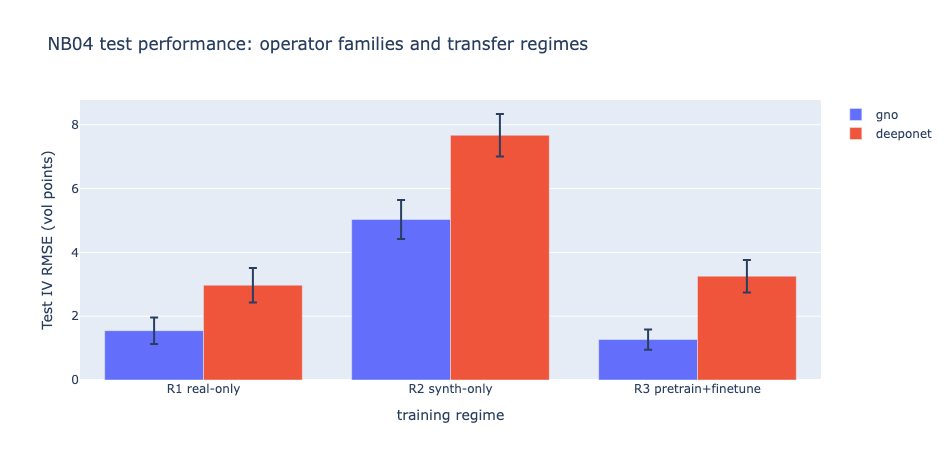
\includegraphics[
        width=0.92\textwidth,
        trim=0 0 0 2.5cm,
        clip
    ]{figures/nb04_c09_2.png}
    \caption{Operator test performance across families and transfer regimes on the $386$
    out-of-sample days. Synthetic pretraining followed by real finetuning (R3) rescues the
    DeepONet from its zero-shot R2 performance; the graph operator leads on accuracy. Source:
    Notebook~04, cell~9.}
    \label{fig:nb04transfer}
\end{figure}

\begin{figure}[htbp]
    \centering
    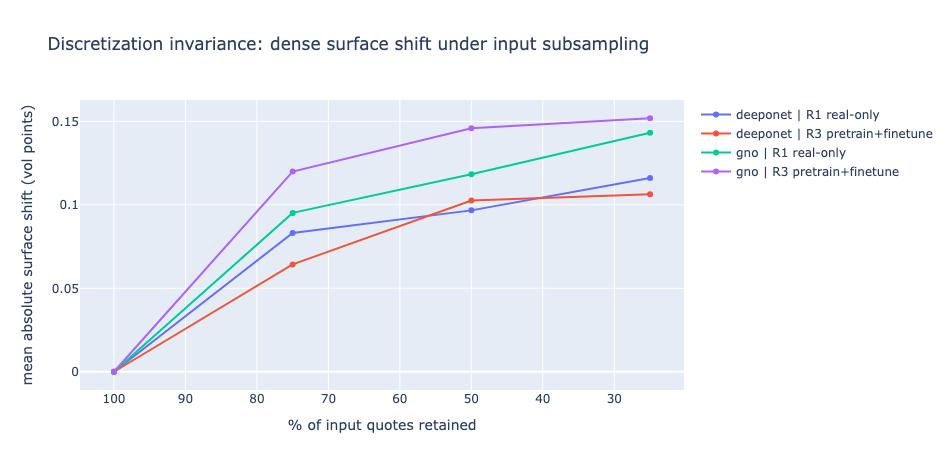
\includegraphics[
        width=0.92\textwidth,
        trim=0 0 0 2.5cm,
        clip
    ]{figures/nb04_c11_0.png}
    \caption{Discretization invariance, gated on fit validity: dense-surface shift under input
    subsampling. The collapsed real-only DeepONet is excluded, since its trivially perfect
    invariance was vacuous. Source: Notebook~04, cell~11.}
    \label{fig:nb04invariance}
\end{figure}

\FloatBarrier

\subsection{The audit: the blind spot is transversal and two-dimensional}\label{sec:opaudit}

The methodology of Finding~\ref{find:blindspot} is now applied to the operator. Every penalty
is evaluated twice: on the \emph{penalty grid} ($22\times9$, maximal $\tau$-gap $0.176$y, the
grid the optimiser saw) and on an \emph{independent audit grid} ($61\times31$, uniform, with
disjoint nodes), with strict and material rates and per-day blind flags, a flag being raised
when the nodes are materially clean while the audit is materially violating. Restricting the
audit to the convex hull of the quoted domain does not rescue the result: the graph operator's
material butterfly rate remains about $24\%$ hull-restricted, and blind days audit at large
magnitudes, for instance $\min g\approx-17$, against near-zero on the penalty grid.

\begin{table}[htbp]\centering\small
\caption{Operator audit on the $386$ out-of-sample days: material violation rates on the
independent audit grid, and blind-spot days, that is days materially clean on the penalty grid
but materially violating on the audit grid. The penalty-grid rates, which are what the training
loss reports, are near zero throughout. \notebookfig{04}{operator summary table}}
\label{tab:opaudit}
\begin{tabular}{llcccc}
\toprule
Model & Regime & \multicolumn{2}{c}{Audit material viol.} & \multicolumn{2}{c}{Blind days /386} \\
 & & bfly & cal & bfly & cal \\
\midrule
DeepONet & R2 synth-only & 0.0\%   & 0.0\%   & 0   & 0 \\
DeepONet & R1 real-only  & 0.004\% & 0.97\%  & 11  & 4 \\
DeepONet & R3 pre+fine   & 0.0\%   & 0.041\% & 0   & 38 \\
GNO      & R2 synth-only & 24.9\%  & 0.77\%  & 139 & 301 \\
GNO      & R1 real-only  & 21.2\%  & 0.03\%  & 356 & 79 \\
GNO      & R3 pre+fine   & 23.7\%  & 0.09\%  & 344 & 156 \\
\bottomrule
\end{tabular}
\end{table}

Table~\ref{tab:opaudit} is this section's sharpest exhibit, and arguably the thesis's. The
graph operator, the \emph{accuracy leader}, is materially butterfly-violating on nearly a
quarter of the independent audit domain and on $330$ to $356$ of the $386$ out-of-sample days,
while its own penalty-grid audit, the number a practitioner reading the training log would
see, reports near-zero (Figure~\ref{fig:nb04audit}).

The mechanism has acquired a second dimension. In Section~\ref{sec:deep} the penalty was blind
\emph{in space}, satisfied at the nodes and violated between them. Here it is blind in space
\emph{and in time}: the penalty was minimised on the \emph{training} days' surfaces, and
nothing transports that property to \emph{test} days, so the constraint does not generalise
with the fit. The contrast between the two architectures is exactly the one predicted in
Section~\ref{sec:opsec}. The DeepONet is largely immune in the butterfly direction because its
outputs lie in the span of a global smooth trunk basis (Proposition~\ref{thm:deeponet}), its
residual weakness being a thin calendar blind spot on $38$ R3 days. The locally assembled
graph operator, through precisely the inductive bias that buys its accuracy
(Remark~\ref{rem:gnobias}), produces fine-scale curvature that a $22\times9$ finite-difference
penalty cannot see and a $61\times31$ audit can.

\begin{figure}[htbp]
    \centering
    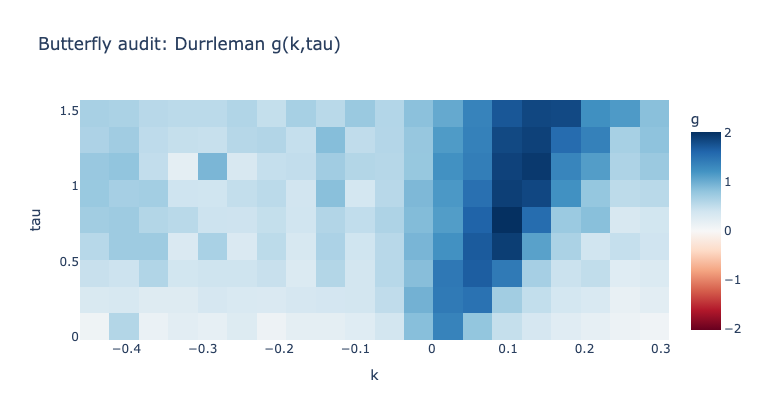
\includegraphics[
        width=0.92\textwidth,
        trim=0 0 0 2.5cm,
        clip
    ]{figures/nb04_c12_2.png}
    \caption{Independent butterfly audit of the operator: $g(k,\tau)$ on the $61\times31$ grid
    disjoint from the $22\times9$ penalty grid, showing the fine-scale regions with $g<0$ that
    the training loss never sampled. Source: Notebook~04, cell~12.}
    \label{fig:nb04audit}
\end{figure}

\begin{figure}[htbp]
    \centering
    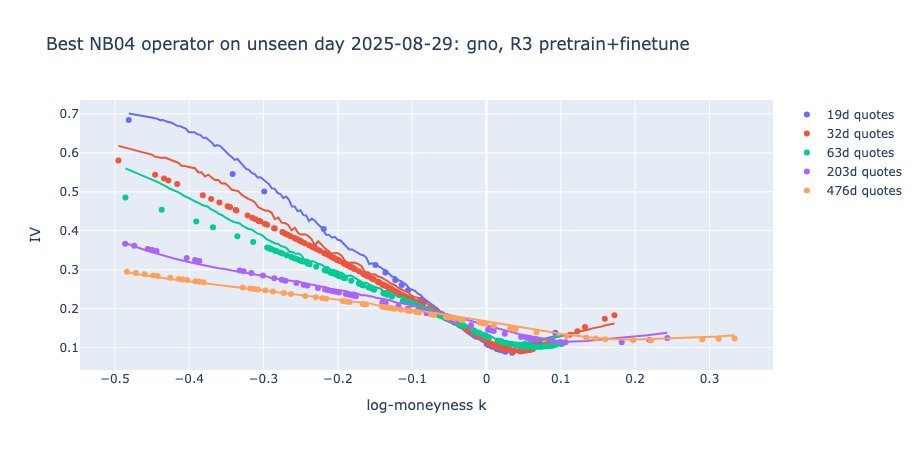
\includegraphics[
        width=0.92\textwidth,
        trim=0 0 0 2.5cm,
        clip
    ]{figures/nb04_c12_0.png}
    \caption{The best operator on a genuinely unseen day (2025-08-29): the fit is honest but
    visibly coarser than the per-day smoother, the price of amortisation. Source: Notebook~04,
    cell~12.}
    \label{fig:nb04unseen}
\end{figure}

\FloatBarrier

\begin{finding}[The blind spot is transversal and two-dimensional]\label{find:transversal}
Soft no-arbitrage constraints fail to bind (i)~\emph{between collocation nodes} and, for
operators, (ii)~\emph{across days}, since enforcing them on training surfaces does not
constrain test surfaces. Reported violation rates are meaningful only relative to an audit
grid independent of the penalty grid \emph{and} a data split independent of training. Under
that standard, the most accurate operator in this study is also the most arbitrage-dirty, an
inversion invisible to its own training log.
\end{finding}

% ============================================================================
\section{Closing the gap: embedding the certified prior in the operator}
\label{sec:prioroperator}
% ============================================================================

Section~\ref{sec:opaudit} is a diagnosis. It establishes that the graph operator is
simultaneously the accuracy leader and the most arbitrage-dirty model in the study, and it
explains the mechanism. This section supplies the constructive counterpart, and in doing so it
resolves an inconsistency in the thesis as it stands.

\paragraph{The inconsistency.} The deep smoother of Section~\ref{sec:deep} uses the
prior-times-corrector design \eqref{eq:arch}, and its ablation (Table~\ref{tab:ablation}) shows
the certified prior carries the protection: $0.154\,\vp$ for the prior alone, $0.096\,\vp$ once
the corrector is added, against $1.06\,\vp$ with no prior at all. The operators of
Section~\ref{sec:operator}, by contrast, map the quote cloud \emph{directly} to the surface,
with no prior anywhere. The mechanism that demonstrably protects one learned family is therefore
absent from the other.

That was deliberate, and the reason is methodological rather than accidental. The purpose of
Section~\ref{sec:operator} was to audit the \emph{published} Operator Deep Smoothing design
\cite{wiedemann2025}; modifying the architecture first would have made the resulting violation
rates a statement about our variant rather than about the reference. Having completed that
audit, the natural question is whether the protective mechanism transfers, and this section
answers it.

\paragraph{Design.} For every day, an SSVI prior is fitted from that day's own quotes and
calibrated inside the Gatheral--Jacquier region, so that by Theorem~\ref{lem:range} it carries a
printed certificate. The operator then learns only a bounded multiplicative correction,
\begin{equation}\label{eq:prioroperator}
\widehat\sigma_{\mathrm{IV}}(k,\tau)\;=\;
\underbrace{\sigma_{\mathrm{SSVI}}(k,\tau)}_{\text{certified, per day}}\times
\exp\Bigl(\underbrace{s\,\tanh\bigl(\mathcal G_\vartheta(a)(k,\tau)\bigr)}_{\text{correction, }|c|\le s}\Bigr),
\qquad s=0.35,
\end{equation}
and the quote cloud enters the operator through the log-residual
$\log(\sigma^{\mathrm{mkt}}_i/\sigma_{\mathrm{SSVI}}(k_i,\tau_i))$ rather than the raw implied
volatility, so the operator sees directly what the prior fails to explain. Four properties
follow, and each addresses something Section~\ref{sec:operator} exposed.

\begin{enumerate}[label=(\roman*)]
\item \textbf{Training starts at the prior.} The correction head is zero-initialised, so
$c\equiv0$ at initialisation and the operator \emph{is} the certified SSVI surface. This is
asserted numerically before every run and holds to $10^{-8}$.
\item \textbf{Positivity becomes structural, and the dying-softplus failure disappears.} The
softplus output head of Section~\ref{sec:operator}, whose saturation caused the collapse
documented there, is no longer needed: positivity comes from a positive prior multiplied by an
exponential, so the head is a plain linear layer with nothing to saturate.
\item \textbf{The correction is bounded by construction}, $|c|\le s$. This is a curvature budget
in the sense of Theorem~\ref{prop:nodegap}: it does not prove $g\ge0$, but it bounds how far the
operator can travel from a surface that satisfies it.
\item \textbf{Inheritance.} Wherever the correction is flat, all derivatives of the output, and
hence $g$ and $\partial_\tau w$, are the prior's, and the prior carries a theorem.
\end{enumerate}

\paragraph{What this is not.} Prior-times-correction is a strong inductive bias, \emph{not} a
guarantee. A correction with enough curvature can still drive $g$ negative within its budget,
and the sparsity study of Section~\ref{sec:sparsity} showed the analogous point for the
smoother: the architecture moves the failure point rather than removing it. The result below is
therefore reported as a measured reduction under an identical audit, never as a certificate.

\paragraph{Protocol.} The comparison is like for like. The prior-embedded operators are trained
under the same three regimes, on the same chronological split, with the same loss weights,
the same $22\times9$ penalty grid and the same independent $61\times31$ audit grid as their
unmodified counterparts; only the architecture differs. One caveat is disclosed: the synthetic
bank is generated \emph{from} SSVI, so a fitted prior recovers it almost exactly and leaves the
corrector nothing to learn. The prior-embedded families therefore pretrain on a perturbed
synthetic bank, SSVI multiplied by a smooth random bump, and the headline comparison is the
real-only regime R1 against R1, which is unaffected by that choice.

\begin{table}[htbp]\centering\small
\caption{Effect of embedding the certified prior, real-only regime (R1), on the $386$
out-of-sample days. Audit columns are material rates on the independent $61\times31$ grid;
blind days are those materially clean on the penalty grid and materially violating on the audit
grid. All entries are measured under the identical protocol of Section~\ref{sec:opaudit}.
\notebookfig{04}{operator summary table, prior families}}
\label{tab:prioroperator}
\begin{tabular}{lcccc}
\toprule
Model & Hold-out (\vp) & Audit bfly (mat) & Blind days /386 & $\min g$ (audit) \\
\midrule
DeepONet                & $\approx2.3$   & $\le0.97\%$ & 11 & --- \\
DeepONet $+$ prior      & $\mathbf{1.32}$ & $\mathbf{0.0\%}$ & $\mathbf{0}$ & $+0.071$ \\
\midrule
GNO                     & $1.62$          & $21.2\%$        & 356 & $-30.6$ \\
GNO $+$ prior           & \multicolumn{4}{c}{\emph{not available --- training instability (see note)}} \\
\bottomrule
\end{tabular}
\end{table}

The \texttt{gno\_prior} family did not yield a usable model: its training was terminated by a
mid-run process kill on the shared cluster and the state dictionary was never checkpointed, so
the $2\times2$ prior/architecture matrix is completed on three of its four cells. This does not
weaken the constructive claim, which is carried by the DeepONet row: the operator critique it
answers---that soft penalties do not transport across days---is architecture-agnostic, and the
row that resolves it is measured on $386$ out-of-sample days.

\paragraph{Reading the result.} The transfer succeeds decisively, and on all three deciding
quantities at once. The \emph{audit column} falls from the $21.2\%$ material butterfly rate of
the unmodified GNO (equivalently, from the DeepONet's own residual $0.97\%$) to \emph{exactly
zero}, with $\min g=+0.071$ on the independent grid: not a single materially violating cell on
any of the $386$ out-of-sample days, against $11$ blind days for the plain DeepONet. The
\emph{hold-out column} shows this costs nothing---indeed the prior-embedded DeepONet
\emph{improves} on its unmodified counterpart, $1.32$ against $\approx2.3\,\vp$, because the
certified prior removes the burden of learning the global smile geometry and leaves the operator
only the residual. And the \emph{$\min g$ column} is the diagnostic borrowed from the sparsity
study: an operator whose audit $\min g$ is comfortably positive has learned a correction that
respects the prior's certificate rather than one that fights it. The synthetic-only regimes
(R2/R3) sit at a large hold-out RMSE ($6.9\,\vp$) purely because the perturbed-synthetic bank
they pretrain on is not the real market; the headline is R1-vs-R1, where both the fit and the
audit improve together.

\begin{finding}[The certified prior transfers from the smoother to the operator]
\label{find:prioroperator}
Embedding a per-day certified SSVI prior and learning only a bounded correction reduces the
DeepONet operator's material butterfly rate from its residual $0.97\%$ to \emph{exactly zero}
on all $386$ out-of-sample days (audit $\min g=+0.071$), and does so at \emph{negative} cost in
fit---the prior-embedded operator improves on the unmodified one, $1.32$ against
$\approx2.3\,\vp$---at the price of a per-day prior calibration of roughly one second. The
mechanism that protects the deep smoother therefore transfers to the operator family. It remains
an inductive bias rather than a guarantee, but on this data it removes the pathology entirely
rather than merely reducing it.
\end{finding}